%
% ======================================================================
\RequirePackage{docswitch}
% \flag is set by the user, through the makefile:
%    make note
%    make apj
% etc.
\setjournal{\flag}

\documentclass[\docopts]{\docclass}

% You could also define the document class directly
%\documentclass[]{emulateapj}

% Custom commands from LSST DESC, see texmf/styles/lsstdesc_macros.sty
\usepackage{lsstdesc_macros}
\usepackage{graphicx}
\graphicspath{{./}{./figures/}}
\bibliographystyle{apj}
\usepackage{subcaption}

% Add your own macros here:
    \usepackage{etoolbox}
    \usepackage{stackengine}
        \setcounter{secnumdepth}{4}

%
% ======================================================================

\begin{document}

\title{ LSST Catalog-level Realization of Gravitationally-lensed Quasars }

\maketitlepre

\begin{abstract}

The scale of the LSST dataset will be such that we should anticipate
extracting as much information out of the its catalogs as possible,
before ever turning to the pixel-level data. In this work we explore the
use of simple, low-multiplicity Gaussian mixture models for realizing
gravitational lens systems in LSST catalog space, to enable both
large-scale sample simulation and direct model inference.

\end{abstract}
% Keywords are ignored in the LSST DESC Note style:
\dockeys{methods: statistical, cosmology: gravitational lenses}

\maketitlepost

% ----------------------------------------------------------------------

\section{Introduction}
\label{sec:intro}

The Large Synoptic Survey Telescope (LSST), a wide-field survey telescope with the diameter of 8.4m, will be start running in Chile in 2020 \cite{LSST_overall}. This telescope has a 3.5 $deg$ of field of view, would cover around 30000 $\textit{deg}^2$ in the sky, and uses $u$, $g$, $r$, $i$, $z$, and $y$ filters \cite{LSSTScienceBookv2}. The telescope will give extensive amount of astronomical data that could be used for the study of Solar System, Extragalactic structures, near-Earth astroids, radiant radio sources, Dark Matter, and Dark Energy \cite{LSSTScienceBookv2}. 

LSST Dark Energy Science Collaboration (DESC) also anticipate to detect around 7000 strongly lensed systems that will procide useful information such as cosmological time delay or lense mass distribution \cite{DESC_overall} \cite{TimeDelayOverall} \cite{Twinkles}. In order to do so, finding the lensed system among the enormous set of data is crucial. However, considering the amount of the data that LSST will produce, pixel-level data searching will be really inefficient and expensive. In order to solve the problem, we propose the lens classification with catalog-level searching with machine learning techniques.

The attempt to use Machine Learning to detect lensed system is not a completely new idea. \citep{convolution_neural_network} suggests that morphological classification of the lensed system using the Convolutional Neural Network(CNN) would be effective. \citep{LensExtractor} has developed 'lensextractor' that uses convolution neural network to train and test the software to detect the lensed system. Most of the previous attemps involved single-band image classification \cite{LensExtractor} \cite{convolution_neural_network}.

We here propose to build a software 'SL Realizer' that does catalog-level lens search to detect lensed system. The 'SL Realizer' project largely consists of two major parts: producing large-sized catalogs of lensed systems and making the software to classify objects in the catalog as lenses or non-lenses. 

We first generated a huge, complete catalog using OM10 lenses \citep{OM10} by calculating the synthetic magnitude of the simulated OM10 lenses. The results are included in \ref{sssec:Synthetic}. Overall, the mock lenses did represent the popluation of the real lenses. We then also calculated the zeroth, first, and the second moment for the OM10 lenses. We used the gaussian fitting method to calculate those moments. The visualization of the lensed system using the moments can be viewed in \ref{fig:visualization}. These OM10 lenses were used as our test set.

We first fitted the model parameters to the catalog-level data using Gaussian Mixture Modeling method. Gaussian Mixture Modeling 

\textit{we should include short summary from the SL Realizer training method}.

In order to validate our model, we used the catalog from the twinkel project \cite{Twinkles}.

\textit{short summary of the result. what we achived}
 
\textit{To be updated after the completion of \ref{sec:sl_realizer_train} at the end of the summer}

%https://arxiv.org/pdf/1705.05857.pdf
%Going through the entire pixel data would be really costly. 

%Very short summary of problem.
%Short discussion of previous attempts to solve it.
%Short description of our new idea.

% In this Note we answer the following questions:
% \begin{itemize}
%  \item How important is ... ?
%  \item With what precision can we ... ?
%  \item What implications does ... have?
%\end{itemize}

%Note on any conventions and assumptions made throughout the paper (magnitude systems, cosmological parameters, etc).

% ----------------------------------------------------------------------

\section{Catalog Generation}
\subsection{Synthetic magnitude calculation}
\label{sssec:Synthetic}

The OM10 mock lensed quasar catalog qso\textunderscore mock.fits contains estimates of the lens galaxy i-band magnitudes, based on a simple Faber-Jackson scaling. With the lenspop library we can compute synthetic magnitudes in i, g, r, and z filters. We validated the computation by plotting the difference in redshift,  i-band magnitude, g-r magnitude, r-i magnitude, and i-z magnitude by

\begin{itemize}
  \item comparing the synthetic magnitudes of the colored OM10 lens galaxies with those of SDSS LRGs.
  \item comparing the synthetic magnitudes of colored OM10 lens galaxies with those of 56 candidate galaxy-scale lenses that were imaged as part of the Canada-France-Hawaii Telescope (CFHT) Legacy Survey.
  \item comparing the synthetic magnitudes of colored OM10 lensed quasars with those of known SDSS Quasars.
\end{itemize}

 \ref{fig:comparison} contains the summary of the validations of synthetic magnitude calculation results, and more data could be viewed directly from our github repository : \url{https://github.com/drphilmarshall/OM10/blob/master/notebooks/Color%20Comparison.ipynb}. All the OM10 lenses were weighted in order to match the distribution of the real population. 
 
 For \ref{fig:lens_sdss}, the two distributions of the real and the mock lenses agreed in 0.63 sigma level. For \ref{fig:lens_cfht}, the two distributions agreed in 0.08 sigma level. For \ref{fig:quasar_sdss}, the two distributions agreed in 0.83 sigma level. The mock lens distributions do represent the real distributions, and we used these mock OM10 lenses as out training set for SL Realizer.
 
\begin{figure}
    \centering
    \begin{subfigure}[b]{0.3\textwidth}
        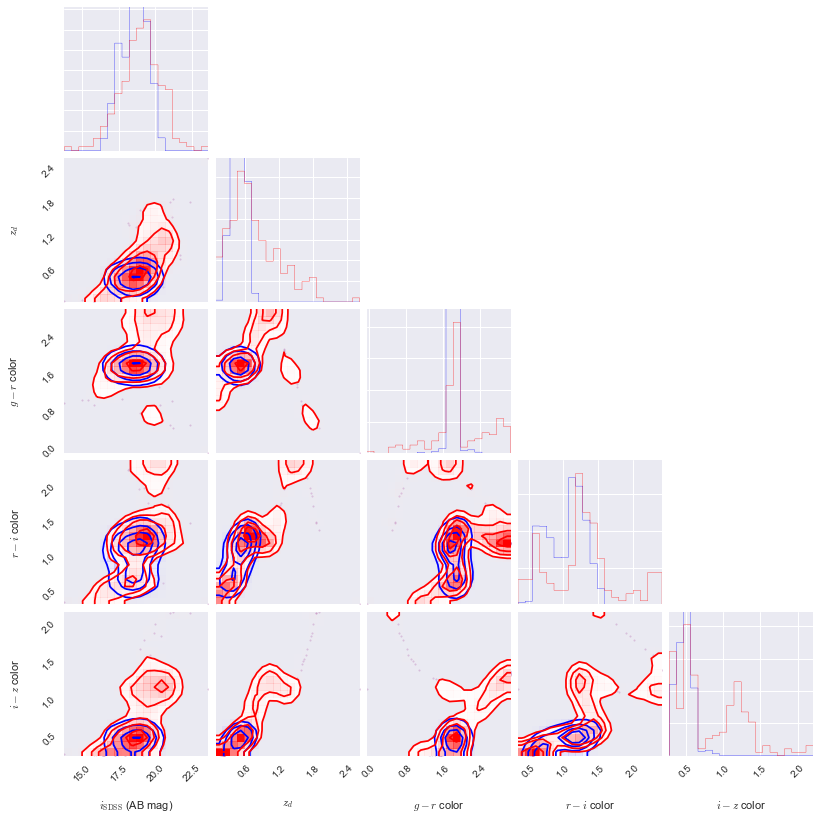
\includegraphics[width=\textwidth]{cfht_om10.png}
        \caption{Comparing the magnitudes between OM10 lenses and CFHT lenses.}
        \label{fig:lens_sdss}
    \end{subfigure}
    ~ %add desired spacing between images, e. g. ~, \quad, \qquad, \hfill etc. 
      %(or a blank line to force the subfigure onto a new line)
    \begin{subfigure}[b]{0.3\textwidth}
        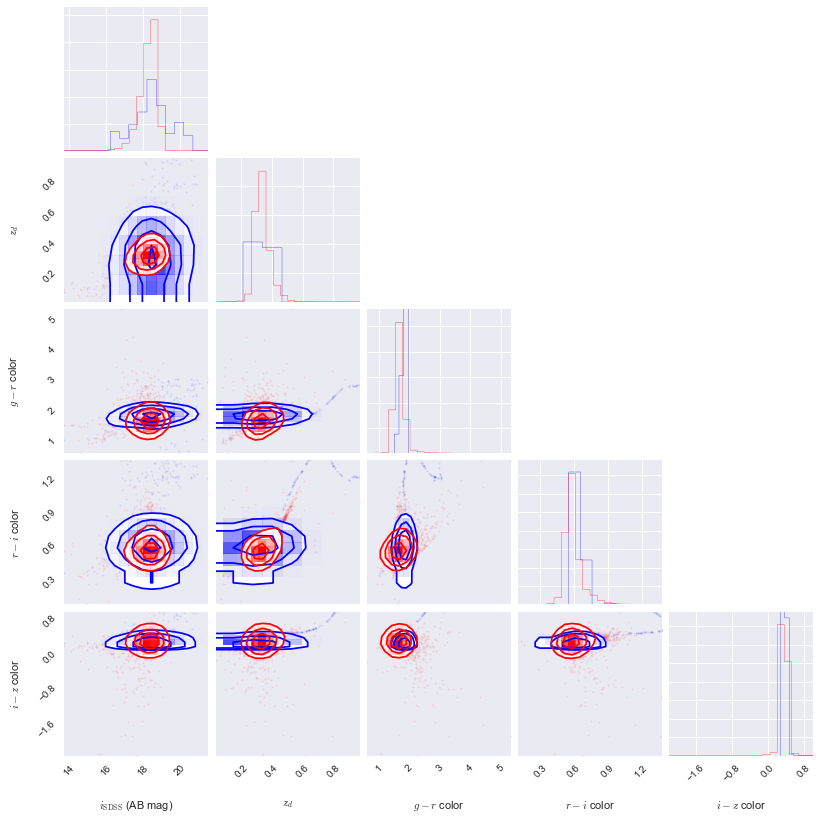
\includegraphics[width=\textwidth]{om10_sdss.png}
        \caption{Comparing the magnitudes between OM10 lenses and CFHT lenses.}
        \label{fig:lens_cfht}
    \end{subfigure}
    ~ %add desired spacing between images, e. g. ~, \quad, \qquad, \hfill etc. 
    %(or a blank line to force the subfigure onto a new line)
    \begin{subfigure}[b]{0.3\textwidth}
        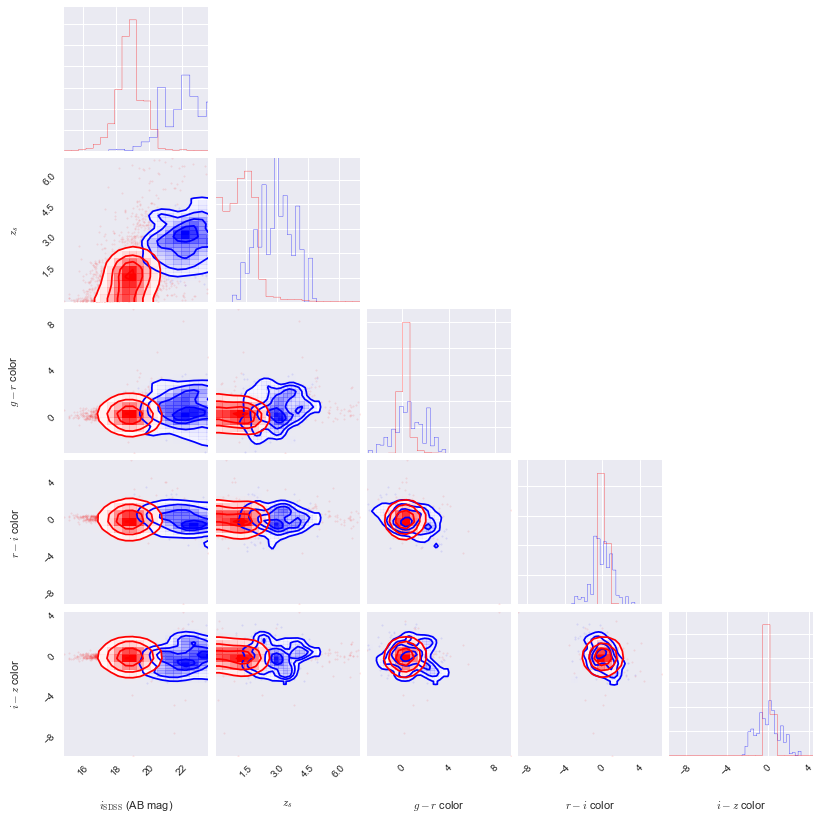
\includegraphics[width=\textwidth]{quasar_sdss.png}
        \caption{Comparing the magnitudes between OM10 quasar sources and SDSS sources. The differences were from the selection effect of SDSS quasras.}
        \label{fig:quasar_sdss}
    \end{subfigure}
    \caption{Comparing OM10 data with SDSS and CFHT data set. }\label{fig:comparison}
\end{figure}

\subsection{Visualization}

Using the OM10 lenses whose magnitude was calculated in
\ref{sssec:Synthetic}, we then visualized the lensed system. Here, in this notebook \url{https://github.com/drphilmarshall/OM10/blob/master/notebooks/Color%20Comparison.ipynb}, we selected a lens system that has a lens ID of $12255151$ and plotted it on different observation epochs. The result can be viewed in \ref{fig:visualization}.

\begin{figure}
    \centering
    \begin{subfigure}[b]{0.2\textwidth}
        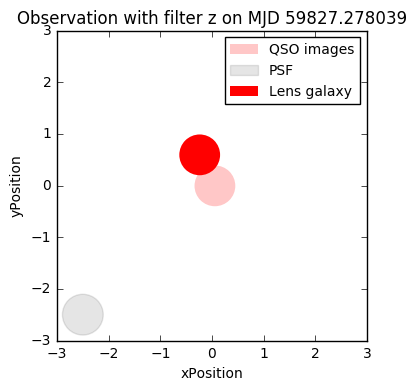
\includegraphics[width=\textwidth]{plot-a.png}
        \caption{Visualizing the lensed system with a filter $z$ on MJD 59827.}
        \label{fig:vis_lens_a}
    \end{subfigure}
    \begin{subfigure}[b]{0.2\textwidth}
        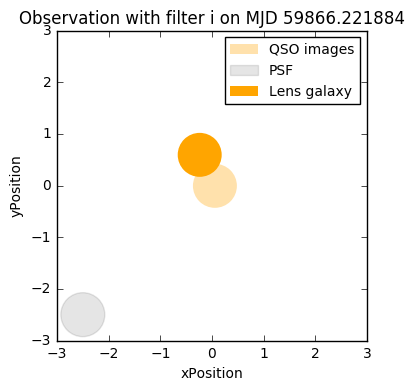
\includegraphics[width=\textwidth]{plot-b.png}
        \caption{Visualizing the lensed system with a filter $i$ on MJD 59866.}
        \label{fig:vis_lens_b}
    \end{subfigure}
    \begin{subfigure}[b]{0.2\textwidth}
        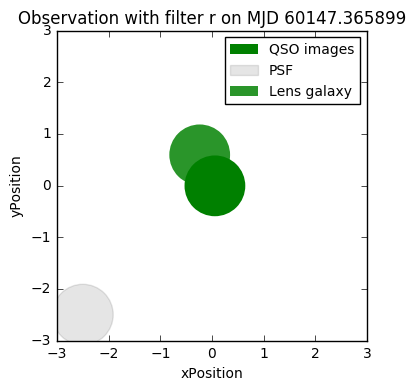
\includegraphics[width=\textwidth]{plot-c.png}
        \caption{Visualizing the lensed system with a filter $r$ on MJD 60147.}
        \label{fig:vis_lens_c}
    \end{subfigure}
    \begin{subfigure}[b]{0.2\textwidth}
        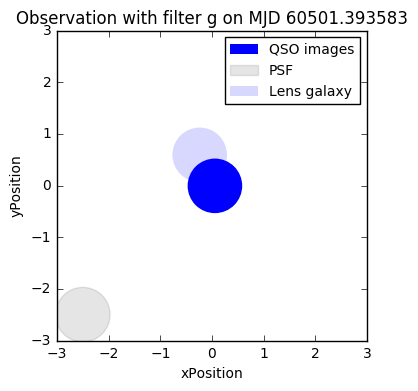
\includegraphics[width=\textwidth]{plot-d.png}
        \caption{Visualizing the lensed system with a filter $g$ on MJD 60501.}
        \label{fig:vis_lens_d}
    \end{subfigure}
    \caption{Visualizing the lensed system(ID $12255151$) in different epochs.}
    \label{fig:visualization}
\end{figure}

\subsection{Mock Catalog Generation}
\label{subsection:MCG}

If we interpret the images of OM10's lensing galaxies and quasars as mixed gaussians, we can simply calculate the zeroth, first, and the second moment of the lensed system. We included these moments in the catalog. The full code for the moment calculation and the catalog generation could be viewed here : \url{https://github.com/jennykim1016/SLRealizer/blob/momentCalc/python/desc/slrealizer/moment.py}.

\subsection{Twinkles Catalog}

The twinkles project also provides the simulation of LSST data \cite{Twinkles}. This project uses LSST's \textit{PhoSim} to generate a mock output of LSST. The table \ref{table:1} contains a few samples of the Twinkles data set. The data set was used as a test set for the SL Realizer.
 
\begin{table}[h!]
\centering
\begin{tabular}{||c c c c c c c||} 
 \hline
 id & ra & dec & magnorm & redshift & majoraxis & minoraxis   \\ [0.5ex] 
 \hline\hline
 21393434 & 53.0524882 & -27.7029739 & 17.8301052 & 0.184 & 1.6126157 & 1.15325373 \\ 
 21393434 & 53.0524882 & -27.7029739 & 17.8301052 & 0.184 & 1.6126157 & 1.15325373 \\
 21393434 & 53.0524882 & -27.7029739 & 17.8301052 & 0.184 & 1.6126157 & 1.15325373 \\
 21393434 & 53.0524882 & -27.7029739 & 17.8301052 & 0.184 & 1.6126157 & 1.15325373 \\
 21393434 & 53.0524882 & -27.7029739 & 17.8301052 & 0.184 & 1.6126157 & 1.15325373 \\ [1ex] 
 \hline
\end{tabular}
\caption{Sample of the Twinkles lensed system data \cite{Twinkles} DATA IS FAKE - NOT THE DATA WE ARE GOING TO USE IN RESEARCH}
\label{table:1}
\end{table}

\label{sec:catalog_generation}

% ----------------------------------------------------------------------

\section{Training SL Realizer}
\label{sec:sl_realizer_train}

Using the catalog level lenses, we would like to train SL Realizer to find the lenses based on the catalog properties. We are aiming to train SL Realizer with the OM10 data set from \ref{sec:catalog_generation} and check the precision with Twinkles data set. 

We can first train the SL Realizer with the known machine learning algorithms. Choosing the right algorithm that will give enough precision without overfitting will be crucial in this step. 

\textit{Some helpful articles for this}

\begin{itemize}
  \item \url{https://www.lsst.org/sites/default/files/docs/137.25_Borne_Data_Mining_Research_8x10.pdf}[LSST data mining overview]
 \item \url{https://arxiv.org/pdf/1608.04369.pdf} [convolutional neural network to differentiate galaxies and stars] The problem is we are not using the pixels to analyze the data
 \item \url{https://arxiv.org/pdf/1703.02642.pdf} [CMU DeepLens] , a new strong gravitational lens finder based on the most recent advances in Deep Learning that still goes through the images. This also uses convolutional neural network
  \item \url{http://www.mpia.de/homes/calj/amla_ss2009/introduction.pdf} [Applications of Machine Learning in Astronomy]
  \item \url{https://arxiv.org/pdf/0906.2173.pdf}[DATA MINING AND MACHINE LEARNING IN ASTRONOMY]
  \item \url{https://academic.oup.com/mnras/article-lookup/doi/10.1093/mnras/stu642}[Skynet]
  \item \url{https://www.analyticsvidhya.com/blog/2015/08/common-machine-learning-algorithms/} [Machien learning techniques]
  
\end{itemize}

We can also use GMM (Gaussian Mixture Model) to link the fitted parameters and the catalog properties. We could also produce a diagram such as \ref{fig:example} that shows how the lensed systems are distributed.

\begin{figure}
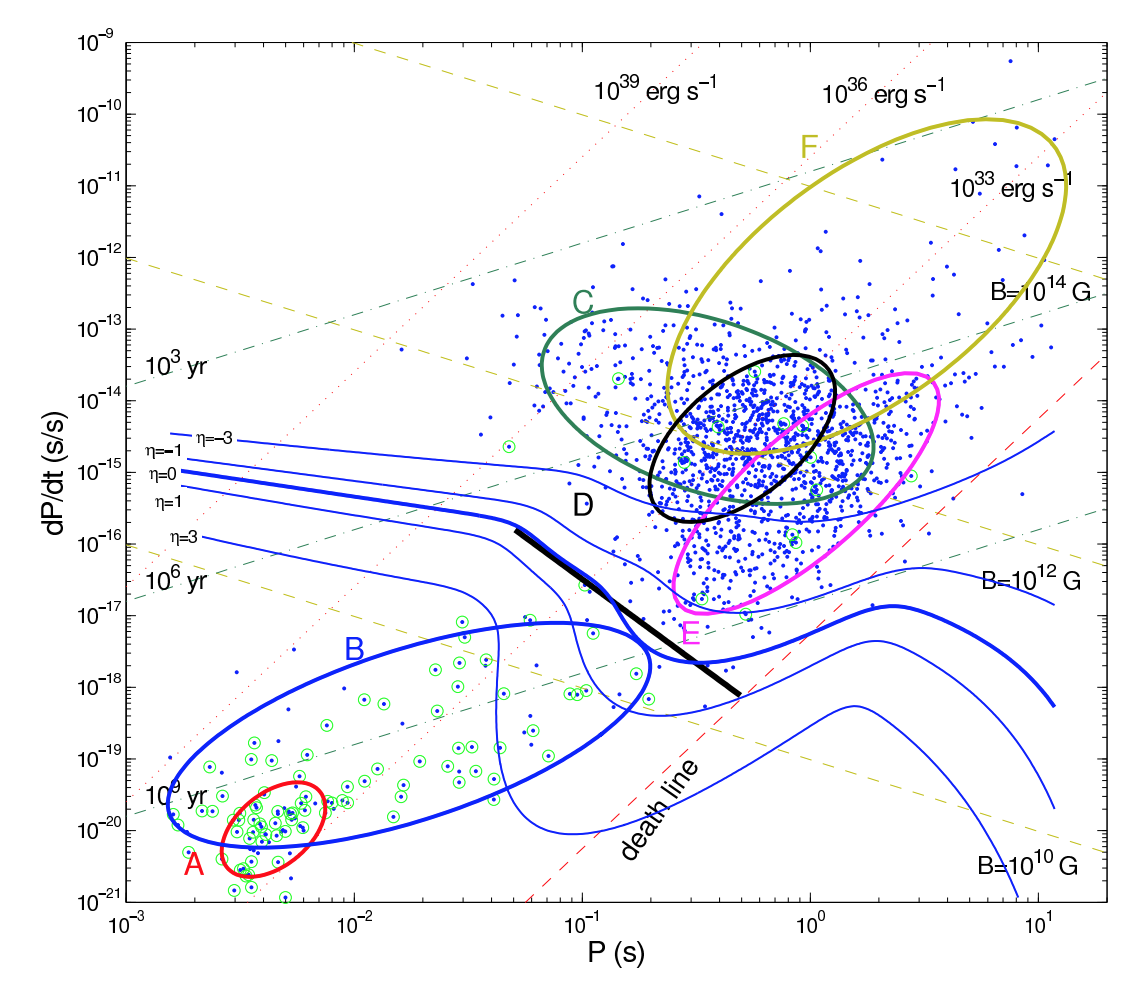
\includegraphics[width=0.3\columnwidth]{PPDiagram.png}
\caption{An example of a diagram that we can produce after GMM.}
 \label{fig:example}
\end{figure}

\textit{The followings discuss GMM.}

\begin{itemize}

\item \url{http://scikit-learn.org/stable/modules/mixture.html}[Gaussian Mixture Model]
\item \url{https://arxiv.org/pdf/1205.6221.pdf}[application of GMM to find pulsars. Nice P-P diagram included]
\end{itemize}



\textit{Using the simulated data from \ref{sssec:Synthetic}, this is what I am going to do during the summer! Result is going to come out soon }

% ----------------------------------------------------------------------

\section{Conclusions}
\label{sec:conclusions}

Here's a summary of what we just reported.

We can draw the following well-organized and neatly-formatted conclusions:
\begin{itemize}
  \item This is important.
  \item We can measure some number with some precision.
  \item This has some implications.
\end{itemize}

Here are some parting thoughts.

% ----------------------------------------------------------------------
% GUIDELINES FROM THE NOTE TEMPLATE:
%
% \section{Introduction}
% \label{sec:intro}
%
% This is a paper and note template for the LSST DESC \citep{Overview,ScienceBook,WhitePaper}.
% You can delete all this tutorial text whenever you like.
%
% You can easily switch between various \LaTeX\xspace styles for internal notes and peer reviewed journals.
% Documents can be compiled using the provided \code{Makefile}.
% The command \code{make} with no arguments compiles \code{main.tex} using the  \code{lsstdescnote.cls} style.
% If you want to upgrade your Note into a journal article, just choose a journal name, between \code{make apj} (ApJ preprint format), \code{make apjl} (which uses the \code{emulateapj} style), \code{make prd}, \code{make prl}, and \code{make mnras}.
%
%
% % ----------------------------------------------------------------------
%
% \section{Commands}
% \label{sec:commands}
%
% There are a number of useful \LaTeX\xspace commands predefined in \code{macros.tex}.
% Notice that the section labels are prefixed with \code{sec:} to allow the use of the \verb=\secref= command to reference a section (\ie, \secref{intro}).
% Figures can be referenced with the \verb=\figref= command, which assumes that the figure label is prefixed with \code{fig:}.
% In \figref{example} we show an example figure.
% You'll notice that the actual figure file is found in the \code{figures} directory.
% However, because we have specified this directory in our \verb=\graphicspath= we do not need to explicitly specify the path to the image.
%
% The \code{macros.tex} package also contains some conventional scientific units like \angstrom, \GeV, \Msun, etc. and some editorial tools for highlighting \FIXME{issues}, \CHECK{text to be checked}, \COMMENT{comments}, and \NEW{new additions}.
%
%
% % ----------------------------------------------------------------------
%
% \section{Methods}
% \label{sec:methods}
%
% Similar to the figure before, here we have included a table of data from \code{tables/table.tex}.
% Notice that again we are able to reference \tabref{example} with the \verb=\tabref= command using the \code{tab:} prefix.
% Also notice that we haven't needed to specify the full path to the table because in the \code{Makefile} we include \code{./tables} directory in the \code{\$TEXINPUTS} environment variable.
%
% \begin{table}
  \begin{center}
  \caption{Example table. \label{tab:example}}
  %\begin{ruledtabular}
  \begin{tabular}{lccc}
\hline\hline
Column 1 & Column 2 & Column 3 &  Column 4 \\[3pt]  
     &    $\deg$     & $\kpc$   &  $\deg$ \\[4pt]
\hline
Obj1 & (0,0) & 10 & 0.1 \\
... & ... & ... & ... \\
ObjN & (0,0) & 10 & 0.1
\\\hline\hline
\end{tabular}
\end{center}
%\end{ruledtabular}
\end{table}

%\begin{\tabletype}{l ccccccc }
%\tablewidth{0pt}
%\tabletypesize{\tiny}
%\tablecaption{ An example table. \label{tab:example}}
%\tablehead{
%(1) & (2) & (3) & (4) & (5) & (6) & (7) & (8)\\
%Name & GLON,GLAT & Distance & $r_{1/2}$ & $\log_{10}(J_{\rm meas})$ & $\log_{10}(J_{\rm pred})$ & Sample & Refrence \\
% & (deg) & (kpc) & (pc) & $\log_{10}(\GeV^2 \cm^{-5})$ & $\log_{10}(\GeV^2 \cm^{-5})$ & & 
%}
%\startdata
%Bootes I                     & 358.08,69.62   & 66  & 189  & $18.8 \pm 0.2$ & 18.5           & I,S,C & ... \\
%\\
%...\\
%\\
%Willman 1                    & 158.58,56.78   & 38  & 19   & $19.1 \pm 0.3$ & 18.9           & I,S & ... \\
%\enddata
%{\footnotesize \tablecomments{ (1) The first column. (2) The second column ...}}
%\end{\tabletype}

%
% Equations appear as follows, and can be referred to as, for example, \eqnref{example} -- just as for tables, we use the \verb=\eqnref= command using the \code{eqn:} prefix.
% \begin{equation}
%   \label{eqn:example}
%   \langle f(k) \rangle = \frac{ \sum_{t=0}^{N}f(t,k) }{N}
% \end{equation}
%
%
% % ----------------------------------------------------------------------
%
% \section{Results}
% \label{sec:results}
%
% \figref{example} shows an example figure, referred to with the \verb=\figref= command and the \code{fig:} prefix.
%
% \begin{figure}
% 
\includegraphics[width=0.9\columnwidth]{example.png}
% \caption{An example figure: the LSST DESC logo, copied from \code{texmf/logos/desc-logo.png} into \code{figures/example.png}. \label{fig:example}}
% \end{figure}
%
%
% % ----------------------------------------------------------------------
%
% \section{Discussion}
% \label{sec:discussion}
%
% If you are planning on committing your paper to GitHub, it's a good idea to write your tex as one sentence per line.
% This allows for an easier \code{diff} of changes.
% It also makes sense to think of latex as \emph{code}, and sentences as logical statements, occupying one line each.
% Each line must ``compile'' in the mind of the reader.
%
%
%
% ----------------------------------------------------------------------

\subsection*{Acknowledgments}

Here is where you should add your specific acknowledgments, remembering that some standard thanks will be added via the \code{acknowledgments.tex} and \code{contributions.tex} files.

% 
This is the text imported from \code{acknowledgments.tex}, and will be replaced by some standard LSST DESC boilerplate at some point.
% 


Author contributions are listed below. \\
Jenny Kim: Initial algorithm and code development, wrote paper. \\
Ji Won Park: Improved algorithm and code development, edited paper. \\
Phil~Marshall: Initiated  project, advised on motivation, model construction and testing. \\
Mike~Baumer: Advised on LSST data characteristics, model construction and testing. \\
Steve~Kahn: Advised on LSST data characteristics, model construction and testing. \\
Rahul~Biswas: Advised on LSST observing cadence, catalog characteristics, error model. \\


%{\it Facilities:} \facility{LSST}
% Include both collaboration papers and external citations:
\bibliography{lsstdesc,main}

\end{document}
% ======================================================================
%
